\chapter{Modelado de Redes Porosas}
\label{champ:model}
\bigskip
\barra
\bigskip

\section{Modelo Dual de Sitios y Enlaces}
La representación Modelo Dual de sitios y Enlaces(MDSE) se puede observar en la Figura \ref{fig:dbsm} en la cual se observa la representación de un medio poroso. Existen varias aplicaciones relacionadas con el MDSE algunas de ellas se reportan en \cite{ref8} y \cite{ref10}. En particular los algoritmos presentados en \cite{ref2}, \cite{ref3} y \cite{ref4} para la creación de redes porosas y en \cite{ref7} para la simulación de la porosimetría del mercurio se basan en el MDSE \cite{ref1}. El MDSE define a un material poroso a través de dos tipos de huecos o poros: los sitios y los enlaces como, cada sitio está conectado a $C$ enlaces, donde $C$ es la conectividad de la red. Cada enlace permite la conexión entre dos sitios, en la Figura \ref{fig:dbsm} se puede observar  una representación en dos dimensiones del MDSE. Una red porosa se puede definir como una matriz cubica.\\

Los algoritmos presentados en \cite{ref2}, \cite{ref3} y \cite{ref4} para la creación de redes y en \cite{ref5} para la simulación de la porosimetría del mercurio se basan en Modelo Dual se Sitios y Enlaces(MDSE) \cite{ref1}. 

\begin{figure}[hbtp]
\centering
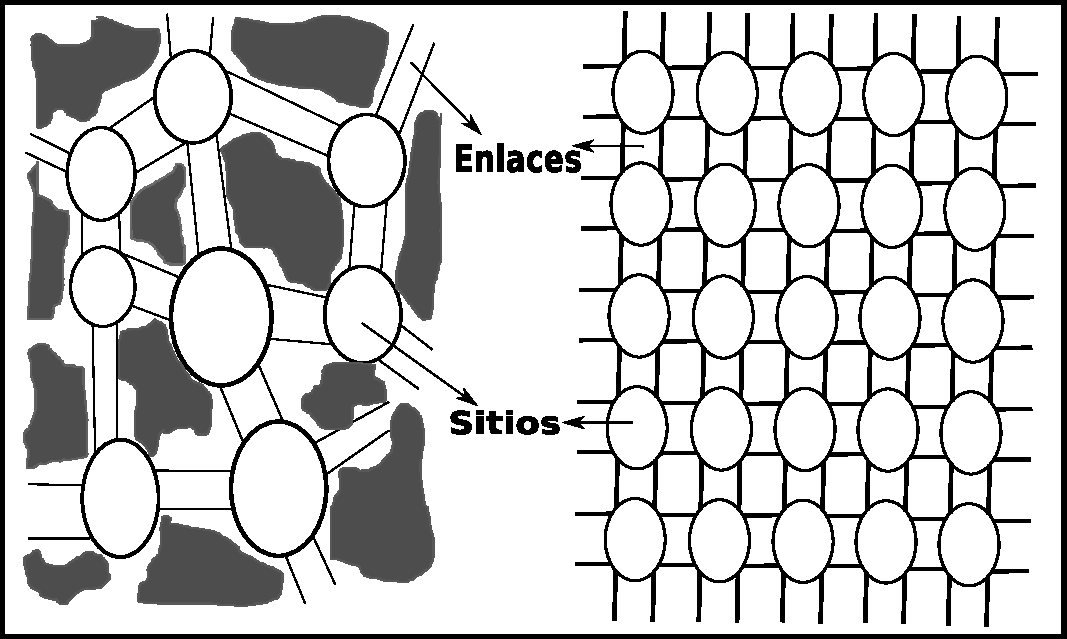
\includegraphics[width=3.5in]{img/dsbm_es.pdf}
\caption{Representación de un material poroso mediante el MDSE}
\label{fig:dbsm}
\end{figure}

 
\section{Principio de Construcción}
Para la creación de redes porosas se tiene el Principio de Construcción ($PC$) el cual establece que: El tamaño de cada sitio debe ser mayor o al menos igual al tamaño de cualquiera de los enlaces conectados al mismo. Los tamaños de los poros se representan a través de dos distribuciones normales $F_S(R_S)$ para los sitios y $F_B(R_B)$ para los enlaces. $R_S$ es el radio de la esfera que representa a los sitios y $R_B$ es el radio del cilindro que representa a los enlaces. Dada las anteriores distribuciones se sabe que si $FS(RS)$ y $F_B(R_B)$ se traslapan, algunos sitios y enlaces tendrán valores iguales. A esta intersección se le conoce como traslape $\Omega$ (Figura \ref{fig:overlap}). El traslape representa la dificultad de que los sitios y enlaces se conecten de una forma válida, respetando el $PC$. Si $\Omega=0$ esto significa que cualquier enlace es menor que cualquier sitio en términos de tamaño lo que significa que la construcción de una red de poros sería muy sencilla. Por el contrario si $\Omega$ es muy cercano a 1, $F_S(R_S)$ y $F_B(R_B)$ serían muy similares por lo que la asignación de enlaces a los sitios estaría más restringida.\\


\begin{figure}[hbtp]
\centering
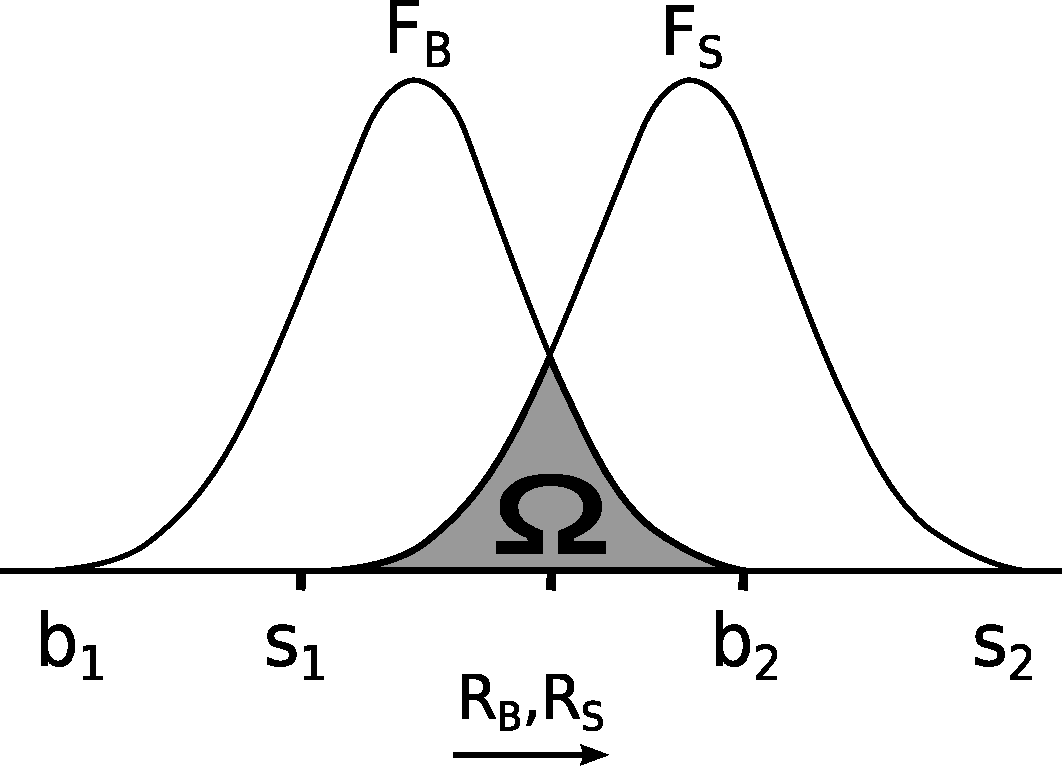
\includegraphics[width=2.5in]{img/traslape.pdf}
\caption{Traslape entre las distribuciones \textit{$F_B$} y $F_S$}
\label{fig:overlap}
\end{figure}

Los algoritmos para la creación de redes porosas definen una red porosa como una matriz cúbica, la cual está formada por la conexión de sitios y enlaces, donde cada sitio se encuentra conectado a tres enlaces directos y a tres enlaces de forma indirecta a través de los sitios vecinos, por lo que se tiene que $C=6$. El tamaño de la red se caracteriza por el parámetro $L$, el cual representa el número de sitos a lo largo de un borde de la matriz cúbica. Con este modelo se tiene que una red de tamaño $L$ contiene $L^3$ sitios y $3L^3$ enlaces (Figura \ref{fig:lattice3d}).

\begin{figure}[hbtp]
\centering
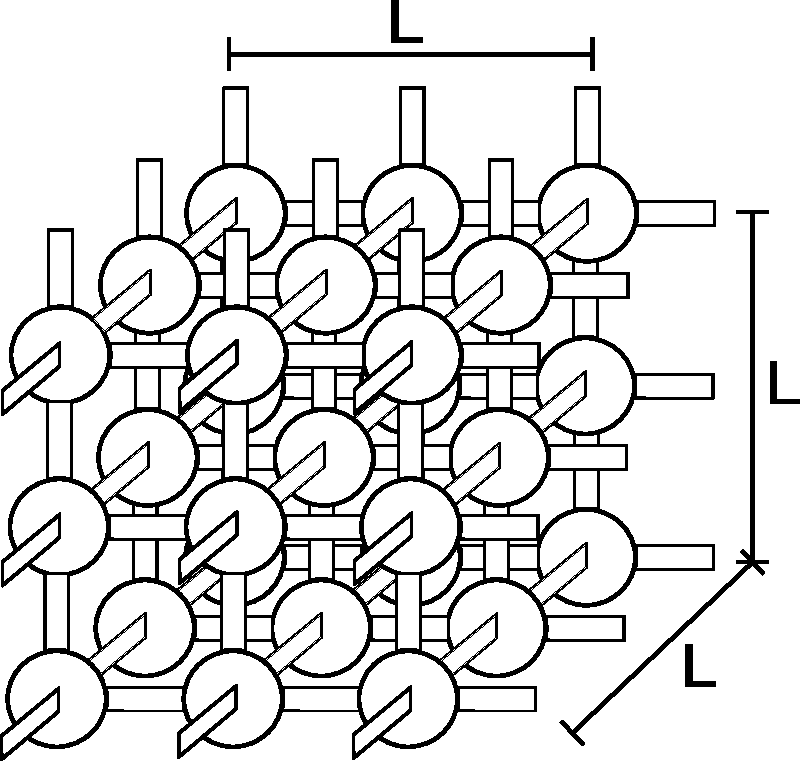
\includegraphics[width=2.8in]{img/red.pdf}
\caption{Red porosas con los sitios representados por esferas y los enlaces representados por cilindros}
\label{fig:lattice3d}
\end{figure}

\section{Restricciones Geométricas}
\label{sec:gr}
Como se menciono anteriormente, para que una red porosa este sujeta a Restricciones Geométricas ($RG$) se debe cumplir para cada enlace conectado aun sitio determinado no debe solaparse con otro enlace conectado al mismo sitio, tal y como se muestra en la Figura \ref{fig:CPyGR}. Las restricciones geométricas surgen cuando se crea una red porosa consistente, mediante el establecimiento de que para cada par de enlaces vecinos conectados a un sitio, la suma de los cuadrados de sus radios debe ser menor (o a lo más igual) que el cuadrado del sitio. Esto se expresa en la Ecuación \ref{eq:eq01}, donde $i$, $j$ varían desde $1$ hasta $6$.\\

\begin{equation}
R_{B}^2[i]+R_{B}^2[j] \leq R_{B}^2
\label{eq:eq01}
\end{equation}

\begin{figure}[hbtp]
\centering
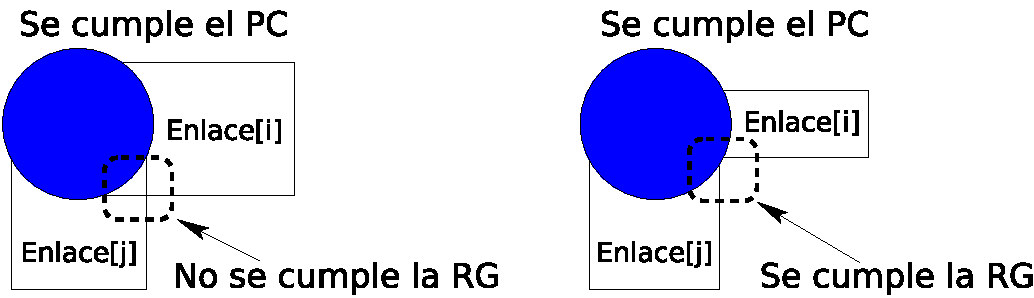
\includegraphics[width=4.0in]{img/CPyGC_es.pdf}
\caption{Representación del $PC$ y $RG$ en un sitio con dos enlaces vecinos}
\label{fig:CPyGR}
\end{figure}
